\documentclass[11pt]{article}
\usepackage[margin=1in]{geometry}
\usepackage{amsmath}
\usepackage{amssymb}
\usepackage{tikz}
\usepackage{pgfplots}
\pgfplotsset{compat=1.18}

\title{Marshallian vs. Hicksian Demand}
\author{ECO 310 Study Guide}
\date{}

\begin{document}

\maketitle

\section{Overview}

There are two fundamental types of demand functions in consumer theory, each answering a different optimization problem.

\begin{center}
\begin{tabular}{|l|l|l|}
\hline
\textbf{Type} & \textbf{Problem} & \textbf{What's Fixed?} \\
\hline
Marshallian & Maximize utility given income & Income $m$ and prices \\
Hicksian & Minimize expenditure given utility & Utility level $\bar{u}$ and prices \\
\hline
\end{tabular}
\end{center}

\section{Marshallian Demand}

\subsection{Definition}

The \textbf{Marshallian demand function} $x^*(p, m)$ solves:
\[
\max_{x} \, u(x) \quad \text{subject to} \quad p \cdot x \leq m
\]

This answers: \textit{``What bundle should I buy to maximize my utility, given my income $m$ and prices $p$?''}

\subsection{Properties}

\begin{itemize}
    \item Depends on \textbf{prices} $p$ and \textbf{income} $m$: $x^*(p, m)$
    \item Also called \textbf{uncompensated demand} (income is not adjusted for price changes)
    \item \textbf{Homogeneous of degree zero}: $x^*(\lambda p, \lambda m) = x^*(p, m)$ (no money illusion)
    \item Satisfies \textbf{Walras' Law}: $p \cdot x^*(p, m) = m$ (consumer spends full budget)
\end{itemize}

\subsection{First-Order Conditions}

At the optimum:
\[
\frac{MU_i}{MU_j} = \frac{p_i}{p_j} \quad \text{for all goods } i, j
\]

Or equivalently: ``bang per buck'' is equalized across all goods:
\[
\frac{MU_i}{p_i} = \frac{MU_j}{p_j}
\]

\subsection{Example: Cobb-Douglas}

For $u(x_1, x_2) = x_1^\alpha x_2^{1-\alpha}$:

\textbf{Marshallian demands:}
\[
x_1^*(p_1, p_2, m) = \frac{\alpha m}{p_1}, \quad x_2^*(p_1, p_2, m) = \frac{(1-\alpha) m}{p_2}
\]

The consumer spends a constant fraction $\alpha$ of income on good 1, and $(1-\alpha)$ on good 2.

\section{Hicksian Demand}

\subsection{Definition}

The \textbf{Hicksian demand function} $h(p, \bar{u})$ solves:
\[
\min_{x} \, p \cdot x \quad \text{subject to} \quad u(x) \geq \bar{u}
\]

This answers: \textit{``What's the cheapest way to achieve utility level $\bar{u}$, given prices $p$?''}

\subsection{Properties}

\begin{itemize}
    \item Depends on \textbf{prices} $p$ and \textbf{target utility} $\bar{u}$: $h(p, \bar{u})$
    \item Also called \textbf{compensated demand} (utility is held constant)
    \item \textbf{Homogeneous of degree zero}: $h(\lambda p, \bar{u}) = h(p, \bar{u})$
    \item By construction: $u(h(p, \bar{u})) = \bar{u}$ (achieves exactly the target utility)
\end{itemize}

\subsection{First-Order Conditions}

At the optimum, the same tangency condition holds:
\[
\frac{MU_i}{MU_j} = \frac{p_i}{p_j}
\]

But now the constraint is $u(x) = \bar{u}$ instead of $p \cdot x = m$.

\subsection{Example: Cobb-Douglas}

For $u(x_1, x_2) = x_1^\alpha x_2^{1-\alpha}$:

\textbf{Hicksian demands:}
\[
h_1(p_1, p_2, \bar{u}) = \bar{u} \left(\frac{\alpha}{1-\alpha}\right)^{1-\alpha} p_1^{-\alpha} p_2^{\alpha-1}
\]
\[
h_2(p_1, p_2, \bar{u}) = \bar{u} \left(\frac{\alpha}{1-\alpha}\right)^{-\alpha} p_1^{\alpha} p_2^{-\alpha}
\]

(These look messy, but the key is they depend on $\bar{u}$ instead of $m$.)

\section{The Expenditure Function}

The \textbf{expenditure function} $e(p, \bar{u})$ is the minimum expenditure needed to achieve utility $\bar{u}$ at prices $p$:
\[
e(p, \bar{u}) = p \cdot h(p, \bar{u})
\]

\textbf{For Cobb-Douglas:}
\[
e(p_1, p_2, \bar{u}) = \bar{u} \cdot p_1^\alpha p_2^{1-\alpha} \left[\alpha^{-\alpha}(1-\alpha)^{-(1-\alpha)}\right]
\]

\section{Relationship Between Marshallian and Hicksian Demand}

The two demand functions are \textbf{dual} to each other. They give the same answer at corresponding income and utility levels.

\subsection{Key Relationship}

If $x^* = x^*(p, m)$ is the Marshallian demand at income $m$, and achieves utility $u^* = u(x^*)$, then:
\[
\boxed{x^*(p, m) = h(p, u^*) \quad \text{and} \quad h(p, \bar{u}) = x^*(p, e(p, \bar{u}))}
\]

In words:
\begin{itemize}
    \item The utility-maximizing bundle at income $m$ equals the cost-minimizing bundle for the utility level you achieve
    \item The cost-minimizing bundle for utility $\bar{u}$ equals the utility-maximizing bundle at the expenditure level $e(p, \bar{u})$
\end{itemize}

\subsection{Graphical Interpretation}

Both problems give the same tangency point:

\begin{center}
\begin{tikzpicture}[scale=1.2]
% Axes
\draw[->] (0,0) -- (5,0) node[right] {$x_1$};
\draw[->] (0,0) -- (0,5) node[above] {$x_2$};

% Indifference curve
\draw[thick, blue, domain=0.5:4.5, smooth, samples=100] plot (\x, {4/\x});
\node[blue, right] at (4.5, 4/4.5) {$u = \bar{u}$};

% Budget line
\draw[thick, red] (0, 4) -- (4, 0);
\node[red, above left] at (0, 4) {Budget: $p \cdot x = m$};

% Optimal point
\filldraw (2, 2) circle (2pt) node[above right] {$x^* = h$};

% Tangency
\draw[dashed] (1.3, 3) -- (2.7, 1);

\end{tikzpicture}
\end{center}

Both the Marshallian problem (maximize utility on the budget line) and the Hicksian problem (minimize cost to reach the indifference curve) give the same tangency point.

\section{Income and Substitution Effects}

The difference between Marshallian and Hicksian demand is crucial for understanding how demand responds to price changes.

\subsection{Slutsky Equation}

When price $p_i$ changes, the total change in Marshallian demand can be decomposed:
\[
\boxed{\frac{\partial x_i^*}{\partial p_i} = \underbrace{\frac{\partial h_i}{\partial p_i}}_{\text{Substitution Effect}} \, \underbrace{- \frac{\partial x_i^*}{\partial m} \cdot x_i^*}_{\text{Income Effect}}}
\]

\begin{itemize}
    \item \textbf{Substitution Effect}: Change in Hicksian demand (pure substitution, utility held constant)
    \begin{itemize}
        \item Always negative: $\frac{\partial h_i}{\partial p_i} < 0$ (law of compensated demand)
    \end{itemize}

    \item \textbf{Income Effect}: How the price change affects purchasing power, and how that affects demand
    \begin{itemize}
        \item Sign depends on whether the good is normal ($\frac{\partial x_i^*}{\partial m} > 0$) or inferior ($\frac{\partial x_i^*}{\partial m} < 0$)
    \end{itemize}
\end{itemize}

\subsection{Graphical Decomposition}

\begin{center}
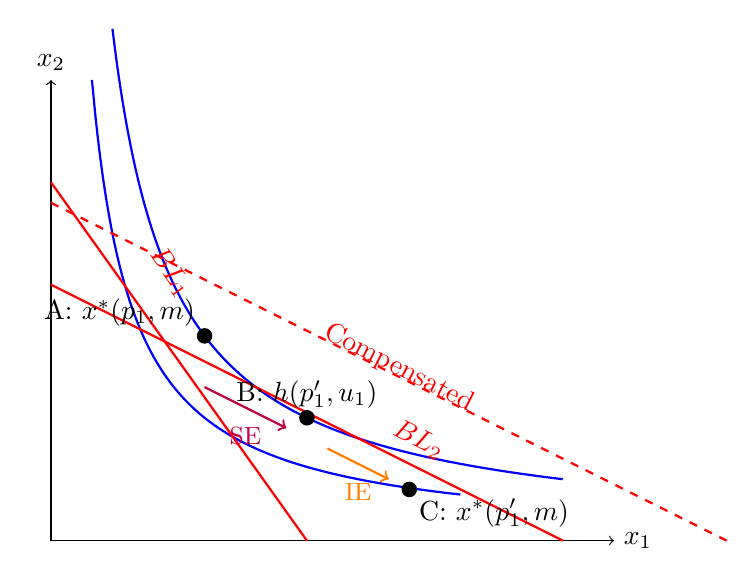
\begin{tikzpicture}[scale=1.3]
% Axes
\draw[->] (0,0) -- (5.5,0) node[right] {$x_1$};
\draw[->] (0,0) -- (0,4.5) node[above] {$x_2$};

% Original indifference curve
\draw[thick, blue, domain=0.6:5, smooth, samples=100] plot (\x, {3/\x});

% New (lower) indifference curve
\draw[thick, blue, domain=0.4:4, smooth, samples=100] plot (\x, {1.8/\x});

% Original budget line (steeper)
\draw[thick, red] (0, 3.5) -- (2.5, 0);
\node[red, above, rotate=-55] at (1, 2.5) {$BL_1$};

% New budget line (flatter - price of x1 fell)
\draw[thick, red] (0, 2.5) -- (5, 0);
\node[red, above, rotate=-27] at (3.5, 0.8) {$BL_2$};

% Compensated budget line (parallel to new, tangent to old IC)
\draw[thick, red, dashed] (0, 3.3) -- (6.6, 0);
\node[red, above right, rotate=-27] at (2.5, 1.9) {Compensated};

% Points
\filldraw (1.5, 2) circle (2pt) node[above left] {A: $x^*(p_1, m)$};
\filldraw (3.5, 0.5) circle (2pt) node[below right] {C: $x^*(p_1', m)$};
\filldraw (2.5, 1.2) circle (2pt) node[above] {B: $h(p_1', u_1)$};

% Arrows
\draw[->, thick, purple] (1.5, 1.5) -- (2.3, 1.1);
\node[purple, below] at (1.9, 1.2) {\small SE};

\draw[->, thick, orange] (2.7, 0.9) -- (3.3, 0.6);
\node[orange, below] at (3, 0.65) {\small IE};

\end{tikzpicture}
\end{center}

When $p_1$ decreases (budget line rotates from $BL_1$ to $BL_2$):
\begin{itemize}
    \item \textbf{A to B}: Substitution effect (compensated) -- always increases demand for good 1
    \item \textbf{B to C}: Income effect -- depends on whether good is normal or inferior
    \item \textbf{A to C}: Total effect = SE + IE
\end{itemize}

\section{Summary Table}

\begin{center}
\begin{tabular}{|l|l|l|}
\hline
\textbf{Feature} & \textbf{Marshallian $x^*(p,m)$} & \textbf{Hicksian $h(p,\bar{u})$} \\
\hline
Problem & Max $u$ s.t. $p \cdot x \leq m$ & Min $p \cdot x$ s.t. $u(x) \geq \bar{u}$ \\
Arguments & Prices $p$ and income $m$ & Prices $p$ and utility $\bar{u}$ \\
Other name & Uncompensated demand & Compensated demand \\
Observable? & Yes (from market data) & No (requires utility info) \\
Price effect & Total = SE + IE & Pure substitution (SE only) \\
Always downward sloping? & No (Giffen goods) & Yes (law of compensated demand) \\
\hline
\end{tabular}
\end{center}

\section{Key Takeaways}

\begin{enumerate}
    \item \textbf{Marshallian demand} is what we observe in real markets -- how much people buy given their income and prices.

    \item \textbf{Hicksian demand} is a theoretical construct that isolates pure substitution effects by holding utility constant.

    \item The two are related through the \textbf{expenditure function}: $h(p, \bar{u}) = x^*(p, e(p, \bar{u}))$

    \item The \textbf{Slutsky equation} decomposes price effects into substitution (Hicksian) and income components.

    \item \textbf{Hicksian demand always slopes down} (compensated law of demand), but Marshallian demand can slope up for Giffen goods (when negative income effect dominates).
\end{enumerate}

\end{document}
